\documentclass{article}

\usepackage{PRIMEarxiv}

\usepackage[utf8]{inputenc} % allow utf-8 input
\usepackage[T1]{fontenc}    % use 8-bit T1 fonts
\usepackage{hyperref}       % hyperlinks
\usepackage{url}            % simple URL typesetting
\usepackage{booktabs}       % professional-quality tables
\usepackage{amsfonts}       % blackboard math symbols
\usepackage{amsmath}
\usepackage{nicefrac}       % compact symbols for 1/2, etc.
\usepackage{microtype}      % microtypography
\usepackage{fancyhdr}       % header
\usepackage{graphicx}       % graphics
\usepackage{enumitem}       % list formatting
\usepackage{algorithm}
\usepackage{float}
\usepackage{algpseudocode}
\usepackage{xcolor}
\usepackage{etoolbox}
\apptocmd{\thebibliography}{\setlength{\itemsep}{1pt}\setlength{\parskip}{0pt}}{}{}
\usepackage{tikz}
\usetikzlibrary{arrows.meta,positioning,fit,backgrounds,calc}
\graphicspath{{figures/}}
\hypersetup{colorlinks=true, linkcolor=cblue, citecolor=cblue, urlcolor=cblue}

% every number in the results comes from scripts/hypotheses/paper_figures.py
\newcommand{\nkappa}{0.1}
\newcommand{\nalpha}{1}
\newcommand{\nfsspQ}{0.691}
\newcommand{\nmckpQ}{0.691}
\newcommand{\nfsspGap}{-0.1}
\newcommand{\nfsspGapLo}{-0.4}
\newcommand{\nfsspGapHi}{0.1}
\newcommand{\nfsspGapTight}{0.8}
\newcommand{\nnaiveGap}{45.3}
\newcommand{\nnaiveGapTight}{71.1}
\newcommand{\nnaiveStarve}{46}
\newcommand{\nalphaZeroGap}{2.6}
\newcommand{\ndspDefaultGap}{33.8}
\newcommand{\nfsspWorstCell}{3.9}
\newcommand{\nfsspWorstCellWhere}{hard-heavy, budget $\times1.5$}
\newcommand{\ndspWorstCell}{10.4}
\newcommand{\nfsspVsDsp}{0.23}
\newcommand{\nfsspVsDspP}{1.5\times10^{-4}}
\newcommand{\nfsspVsNaive}{27.2}
\newcommand{\nfsspVsNaiveP}{5\times10^{-5}}
\newcommand{\nfsspArrMin}{-0.2}
\newcommand{\nfsspArrMax}{1.4}
\newcommand{\nfsspArrfcfs}{0.1}
\newcommand{\nfsspArrrandomfcfs}{-0.1}
\newcommand{\nfsspArrhardesttaskfirst}{1.4}
\newcommand{\nfsspArreasiesttaskfirst}{-0.2}
\newcommand{\nfsspArrmarginalroipriority}{1.0}
\newcommand{\narrfcfs}{23.0}
\newcommand{\narrrandomfcfs}{22.7}
\newcommand{\narrhardesttaskfirst}{29.8}
\newcommand{\narreasiesttaskfirst}{8.9}
\newcommand{\narrmarginalroipriority}{29.7}
\newcommand{\nutbestmodel}{71.1}
\newcommand{\nutmarginalroiratio}{31.4}
\newcommand{\nutquasilinear}{6.0}
\newcommand{\nutshapleybudgetshare}{4.0}
\newcommand{\nutdynamicshadowprice}{0.9}
\newcommand{\ncascadeQ}{0.728}
\newcommand{\ncascadeGap}{7.3}
\newcommand{\nmainMckpQ}{0.691}
\newcommand{\nnoiseDropMckp}{2.0}
\newcommand{\nnoiseDropFssp}{1.9}
\newcommand{\nunKnownGap}{-0.1}
\newcommand{\nunOnlineGap}{0.1}
\newcommand{\nunOnlineWorst}{3.9}
\newcommand{\nunOnlineStarve}{0.1}
\newcommand{\nunOnlineLowGap}{0.0}
\newcommand{\nunOnlineLowWorst}{4.2}
\newcommand{\nunOnlineLowStarve}{0.2}
\newcommand{\nunOnlineHighGap}{0.2}
\newcommand{\nunOnlineHighWorst}{3.7}
\newcommand{\nunOnlineHighStarve}{0.0}
\newcommand{\nunHalfGap}{15.9}
\newcommand{\nunHalfWorst}{39.4}
\newcommand{\nunHalfStarve}{17.7}
\newcommand{\nunThreeQGap}{3.5}
\newcommand{\nunThreeQWorst}{17.7}
\newcommand{\nunThreeQStarve}{4.6}
\newcommand{\nunFiveQGap}{1.3}
\newcommand{\nunFiveQWorst}{8.2}
\newcommand{\nunFiveQStarve}{0.0}
\newcommand{\nunDoubleGap}{3.7}
\newcommand{\nunDoubleWorst}{23.4}
\newcommand{\nunDoubleStarve}{0.0}
\newcommand{\nunOnlineMaxGap}{0.2}
\newcommand{\noracleWorst}{19.3}
\newcommand{\noracleWorstWhere}{hard-heavy, budget $\times1$}
\newcommand{\noracleGap}{2.2}
\newcommand{\nsteepNaive}{44.3}
\newcommand{\nsteepFssp}{-0.5}
\newcommand{\ninfoGainMin}{2}
\newcommand{\ninfoGainMax}{19}
\newcommand{\nfmnaive}{64.7}
\newcommand{\njainnaive}{0.24}
\newcommand{\nfmfssp}{-4.7}
\newcommand{\njainfssp}{0.96}
\newcommand{\nfmdsp}{8.6}
\newcommand{\njaindsp}{0.96}
\newcommand{\njainmckp}{0.96}
\newcommand{\ntotalRuns}{351{,}900}


\definecolor{ours}{HTML}{008300}
\definecolor{cblue}{HTML}{2a78d6}
\definecolor{corange}{HTML}{eb6834}
\definecolor{cgray}{HTML}{52514e}

% Header
\pagestyle{fancy}
\thispagestyle{empty}
\rhead{ \textit{ }}
\fancyhead[LO]{MasBudget: Fair-Share Shadow Pricing for LLM Agents Sharing One Budget}

%% Title
\title{MasBudget: Fair-Share Shadow Pricing\\ for LLM Agents Sharing One Budget}

\author{
  Chauhan Mitesh Vijaybhai, Rathod Yuvraj Rajubhai, Solanki Viraj Rajeshbhai, Sunay Mohit Desai \\
  \texttt{\{chauhan.mitesh, yuvraj.rathod, viraj.solanki, 24110361\}@iitgn.ac.in} \\
}

\begin{document}
\maketitle

\begin{abstract}
Multi-agent AI systems can call language models whose prices differ by two orders of magnitude. When autonomous agents pay for their calls from one shared budget, each agent's choice changes what the others can afford. A central controller can solve this as a knapsack problem, but it needs all tasks up front and is a single point of control. We model the decentralized alternative as a sequential game in which agents arrive one at a time, see the remaining budget, and pick the model that maximizes their own utility. Using real pass/fail and cost data for 1,055 coding tasks and six models from LLMRouterBench, we explore 5 arrival orders and 5 utility functions. Greedy agents lose \nnaiveGapTight\% of the achievable quality at tight budgets, and existing utilities only work if their price parameter is re-tuned for every budget. We then propose \emph{Fair-Share Shadow Pricing} (FSSP), a one-line utility that prices money in units of the budget still available per waiting task. With one parameter setting for all budgets, task mixes and agent counts, FSSP agents reach a mean pass@1 of \nfsspQ{} against \nmckpQ{} for the exact centralized optimum, never starve a task in the realistic setting, and keep fairness at the level of the central planner. It needs no scheduler and no advance knowledge of the number of requests.
\end{abstract}


% ======================================================================
\section{Introduction}

Large language models (LLMs) differ widely in price and skill. In our data a call to \texttt{gemini-2.5-pro} costs about 120 times more than one to \texttt{deepseek-v3.1-terminus}, yet on easy coding tasks both always pass. LLM routers such as RouteLLM, FrugalGPT and MasRouter therefore learn to send each query to a suitable model~\cite{ong2024routellm,chen2023frugalgpt,yue2025masrouter,zhang2026mtrouter}.

The problem changes when \emph{many autonomous agents} share \emph{one} budget (Figure~\ref{fig:system}). Each agent wants a good answer for its own task, but every dollar it spends is a dollar the next agent cannot use. If an early agent buys the frontier model for a task that a cheap model could solve, a later agent with a hard task may find the budget empty. Two designs are possible. A \emph{centralized} controller collects all tasks and solves a global knapsack problem. This is optimal, but it must wait for all tasks, needs full knowledge of them and is a single point of failure. In a \emph{decentralized} design each agent decides for itself when its request arrives. This fits asynchronous pipelines, but it can waste the shared budget.

\begin{figure}[t]
\centering
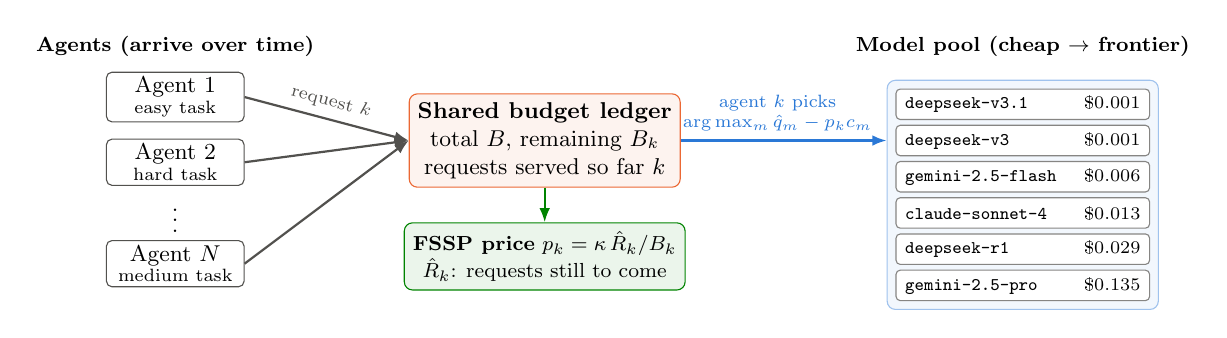
\begin{tikzpicture}[scale=0.92, transform shape,
  font=\small,
  agent/.style={draw=cgray, rounded corners=2pt, fill=white, minimum width=1.9cm, minimum height=0.6cm, align=center, inner sep=2pt},
  model/.style={draw=cgray!70, rounded corners=1.5pt, fill=white, minimum height=0.42cm, inner sep=2pt, font=\scriptsize},
  arr/.style={-{Latex[length=1.8mm]}, thick},
]
% ---- agents (left column)
\node[font=\footnotesize\bfseries] at (0, 2.05) {Agents (arrive over time)};
\node[agent] (a1) at (0, 1.35) {Agent 1\\[-3pt]\scriptsize easy task};
\node[agent] (a2) at (0, 0.45) {Agent 2\\[-3pt]\scriptsize hard task};
\node at (0, -0.25) {$\vdots$};
\node[agent] (an) at (0, -0.95) {Agent $N$\\[-3pt]\scriptsize medium task};
% ---- shared ledger + price (middle column)
\node[draw=corange, fill=corange!8, rounded corners=3pt, minimum width=3.1cm, minimum height=1.25cm, align=center] (bud) at (5.1, 0.75)
  {\textbf{Shared budget ledger}\\ total $B$, remaining $B_k$\\ requests served so far $k$};
\node[draw=ours, fill=ours!8, rounded corners=3pt, minimum width=3.1cm, align=center, font=\footnotesize] (price) at (5.1, -0.85)
  {\textbf{FSSP price} $p_k = \kappa\,\hat R_k/B_k$\\ $\hat R_k$: requests still to come};
\draw[arr, ours] (bud.south) -- (price.north);
% ---- model pool (right column)
\node[font=\footnotesize\bfseries] at (11.7, 2.05) {Model pool (cheap $\rightarrow$ frontier)};
\foreach \name/\cost [count=\i] in {deepseek-v3.1/0.001, deepseek-v3/0.001, gemini-2.5-flash/0.006, claude-sonnet-4/0.013, deepseek-r1/0.029, gemini-2.5-pro/0.135} {
  \node[model, minimum width=3.5cm] (m\i) at (11.7, 1.75-0.5*\i) {\makebox[2.45cm][l]{\texttt{\name}}\makebox[0.8cm][r]{\$\cost}};
}
\begin{scope}[on background layer]
  \node[fit=(m1)(m6), fill=cblue!6, draw=cblue!45, rounded corners=3pt, inner sep=3pt] (pool) {};
\end{scope}
% ---- arrows
\draw[arr, cgray] (a1.east) -- node[above, font=\scriptsize, sloped]{request $k$} (bud.west);
\draw[arr, cgray] (a2.east) -- (bud.west);
\draw[arr, cgray] (an.east) -- (bud.west);
\draw[arr, cblue] (bud.east) -- node[above, font=\scriptsize, align=center, pos=0.47]{agent $k$ picks\\ $\arg\max_m \hat q_m - p_k c_m$} (pool.west |- bud.east);
\end{tikzpicture}
\caption{Agents with tasks of different difficulty share one model budget. In the decentralized setting studied here, each agent decides alone when it arrives. FSSP (Section~\ref{sec:fssp}) gives each agent one price, the inverse of the budget still available per request still to come; $\hat q_m$ is the agent's estimated chance that model $m$ solves its task and $c_m$ the model's price. The centralized alternative we compare against replaces the ledger by one controller that sees all tasks and solves a knapsack problem.}
\label{fig:system}
\end{figure}

We look for a decentralized rule that performs as well as the central controller. We model the interaction as a \emph{sequential resource-allocation game}~\cite{nisan2007algorithmic} whose outcome depends on two design choices, the arrival order and the agents' utility function, and study them with real pass/fail and cost data for 1,055 LiveCodeBench tasks and six commercial models~\cite{llmrouterbench,jain2024livecodebench}.

Our contributions are:
\begin{enumerate}[leftmargin=*, itemsep=1pt]
  \item A controlled benchmark of the decentralized design space (5 arrival orders $\times$ 5 utilities) against five centralized methods, including the exact knapsack optimum, over 8 budgets, 3 task mixes and 50 seeds, with a realistic \emph{expected-quality} information model.
  \item Two findings that guided our design: the utility matters far more than the arrival order, and serving easy tasks first is best while serving hard tasks first is worst. Existing price-based utilities match the optimum only if their price is re-tuned for every budget.
  \item \textbf{Fair-Share Shadow Pricing (FSSP)}, a scale-free, self-correcting utility whose price is the inverse of the remaining budget per waiting task. With one parameter setting it matches the centralized optimum on held-out seeds, stays robust across model pools, information settings, agent counts and noisy labels, and removes the first-mover advantage of greedy agents.
\end{enumerate}

% ======================================================================
\section{Related Work}

LLM routers choose a model per query for one system: RouteLLM trains a strong-vs-weak router~\cite{ong2024routellm}, FrugalGPT escalates from cheap to expensive models when a check fails~\cite{chen2023frugalgpt}, MasRouter routes the agents of one multi-agent system~\cite{yue2025masrouter}, and MTRouter handles a cost budget over multi-turn dialogue~\cite{zhang2026mtrouter}. They decide centrally, while we study self-interested agents that draw from a common budget without a router. On the economics side, shadow prices let independent users share a network~\cite{kelly1998rate}, budget pacing adjusts a bidder's price multiplier as its budget is spent~\cite{balseiro2019learning}, and distributed welfare and cost-sharing games study how local payoffs shape global efficiency~\cite{marden2013distributed,chandan2019optimal}. Greedy rules for submodular problems carry constant-factor guarantees~\cite{nemhauser1978analysis,williams2017decentralised}, and the centralized problem is a multiple-choice knapsack problem (MCKP)~\cite{kellerer2004knapsack}. FSSP borrows the shadow-price idea but normalizes the price by the remaining number of tasks, so it needs no per-budget tuning.

% ======================================================================
\section{Problem Formulation}

There are $n$ jobs. Each of the $N$ agents owns $T$ tasks, so $n = NT$, and every task needs one model call. Model $m$ from the model pool $\mathcal{M}$ costs $c_m$ per call, and $q_{i,m}\in[0,1]$ is the probability that model $m$ solves job $i$. All calls are paid from a shared budget $B$.

\textbf{Centralized benchmark.} A controller that sees all jobs chooses one model (or none) per job, with $x_{i,m}=1$ if job $i$ is given model $m$:
\begin{equation}
\max_{x}\ \sum_{i}\sum_{m} q_{i,m}\,x_{i,m}\quad \text{s.t.}\quad \sum_{i}\sum_{m} c_m x_{i,m}\le B,\quad \sum_m x_{i,m}\le 1,\quad x_{i,m}\in\{0,1\}.
\label{eq:mckp}
\end{equation}

\textbf{Decentralized sequential game.} Jobs arrive in an order $\pi$, where $\pi_j$ is the job served at step $j = 0, 1, \dots$ and $m_{\pi_j}$ the model it bought. At step $k$ the arriving agent observes the remaining budget $B_k = B - \sum_{j<k} c_{m_{\pi_j}}$, may choose any model with $c_m \le B_k$, picks $m_k = \arg\max_{m:\,c_m\le B_k} U(m)$, and pays immediately. If no model is affordable, the job is \emph{starved} and scores 0. The two design levers are the order $\pi$ and the utility $U$.

\textbf{Metrics.} We report the mean realized pass@1 $\bar Q$, the \emph{optimality gap} $(\bar Q_{\text{MCKP}}-\bar Q)/\bar Q_{\text{MCKP}}$ paired on the same instance (the price of anarchy), the share of starved tasks, Jain's fairness index over agent payoffs~\cite{jain1984fairness} (1 = all agents score the same), and the first-mover advantage (mean payoff of the first quarter of agents minus that of the last quarter).

% ======================================================================
\section{Methodology}

\subsection{Benchmark and information model}

We use the \texttt{livecodebench/test} split of LLMRouterBench~\cite{llmrouterbench}: 1,055 code-generation tasks, each run once by six models with a recorded API cost and binary pass@1 (1 if the model's answer passes all unit tests). Model prices are the measured mean cost per call (Figure~\ref{fig:system}). Tasks carry a difficulty label (easy, medium or hard by tertile of mean pass rate). Every model passes every easy task. On medium tasks pass rates range from 0.68 (\texttt{claude-sonnet-4}) to 0.98 (\texttt{deepseek-r1}), and on hard tasks only \texttt{deepseek-r1} and \texttt{gemini-2.5-pro} clearly help (0.43 against 0.06--0.15 for the others).

\textbf{What agents know.} An agent cannot know whether a model will solve its task before calling it. In our main \emph{expected-quality} setting, an agent sees only $\hat q_{i,m}$, the pass rate of model $m$ on the difficulty tier of task $i$. This rate is estimated by 5-fold cross-fitting, so a task's own result is never used for its estimate. All methods, centralized ones included, plan with $\hat q$ and are scored on the real pass/fail outcome. As an upper bound we also report an \emph{oracle} setting in which every method knows the true outcome.

\textbf{Instances.} Each instance has $N{=}10$ agents with $T{=}10$ tasks each, drawn from one of three mixes: uniform (1/3 of each tier), easy-heavy (80/10/10) and hard-heavy (10/10/80). The budget is $B = \beta \cdot c_{\min} \cdot n$, where $c_{\min}$ is the price of the cheapest model and $\beta \in \{1, 1.5, 3, 6, 12, 25, 50, 120\}$ is the budget per task in units of that price. At $\beta{=}1$ every task can afford only the cheapest model, at $\beta{=}120$ the most expensive one. We call $\beta \in\{1.5, 3, 6\}$ \emph{tight} budgets.

\subsection{Methods compared}

\textbf{Centralized.} (i) \emph{Optimal MCKP}: the exact solution of Eq.~\eqref{eq:mckp} with OR-Tools/SCIP. (ii) \emph{Predictive router}: gives every job the cheapest model, then greedily upgrades the job with the best quality gain per dollar. (iii) \emph{Static equal quota}: each agent receives $B/N$ and solves its own knapsack. (iv) \emph{Confidence cascade} in the style of FrugalGPT: tries models from cheap to expensive and stops when the unit tests pass. (v) \emph{Cheapest model} for every job.

\textbf{Decentralized design space.} Arrival orders: round-robin FCFS, uniformly random, hardest-first (HTF), easiest-first (ETF), and marginal-ROI priority (largest $(q_m - q_{\text{cheap}})/(c_m - c_{\text{cheap}})$ first). Here $q_m$ is short for the arriving task's $\hat q_{i,m}$, and $q_{\text{cheap}}, c_{\text{cheap}}$ refer to the cheapest model. Utilities: \emph{best-model} $U=q_m$ (greedy); \emph{quasi-linear} $U = q_m - \lambda c_m$; \emph{dynamic shadow price} $U = q_m - p_0 (B/B_k)^{\alpha} c_m$~\cite{kelly1998rate,balseiro2019learning}; \emph{Shapley budget share} $U = q_m - \frac{\lambda}{1+\gamma\phi_i} c_m$, with $\phi_i$ the Monte-Carlo Shapley value of the agent and $\gamma$ its weight~\cite{chandan2019optimal}; and the \emph{marginal ratio} $U = \frac{q_m - q_{\text{cheap}}}{c_m - c_{\text{cheap}}}$~\cite{williams2017decentralised}. The price parameters ($\lambda$, base price $p_0$, exponent $\alpha$) were tuned on separate tuning seeds, either once for all budgets or separately for each budget level (marked $^*$).

\subsection{From the design space to a new utility}
\label{sec:fssp}

Exploring this design space (Section~\ref{sec:results}) taught us three things about what a good decentralized utility must do.
\begin{enumerate}[leftmargin=*, itemsep=1pt]
  \item \textbf{It must price money at all.} Greedy agents buy \texttt{gemini-2.5-pro} at \$0.135 for tasks that a \$0.001 model solves, and the budget is gone after a few requests.
  \item \textbf{The price must match the budget scale.} With the proposal's default $\lambda=0.5$ the cost term is at most $0.07$ and changes nothing. The best \emph{fixed} $\lambda$ is about $0.07/(B/n)$ for mid-range budgets, and the tuned values span about three orders of magnitude across our budgets. A single $\lambda$ or $p_0$ for all budgets collapses to "always buy the cheapest model".
  \item \textbf{The price should react to how the budget is being spent, not only to how much is left.} The shadow price $(B/B_k)^{\alpha}$ always rises along the queue, even when earlier agents spent exactly their share, so late agents are taxed for being late.
\end{enumerate}

\textbf{Fair-Share Shadow Pricing (FSSP).} These points lead to a simple rule. Requests are numbered by their position in the queue, $k = 0, 1, \dots, n-1$, so when request $k$ arrives, $k$ requests have already been served and paid for, and $n-k$ (this one included) still need a model. Let $b = B/n$ be the initial fair share per request, and let
\begin{equation}
f_k = \frac{B_k}{n-k}
\end{equation}
be the budget still available per waiting request (when $n$ is unknown, $n-k$ is replaced by an estimate $\hat R_k$, see below). The agent that owns request $k$ (its task is job $i$) measures cost in units of this fair share:
\begin{equation}
U_k(m) = \hat q_{i,m} - p_k\,c_m, \qquad p_k = \frac{\kappa}{b}\left(\frac{b}{f_k}\right)^{\alpha},
\label{eq:fssp}
\end{equation}
where $B_k$ is the remaining budget at step $k$, $c_m$ the price of model $m$, $\kappa>0$ the price scale and $\alpha\ge0$ the strength of the scarcity feedback. With the selected $\alpha=\nalpha$ the initial share $b$ cancels and the price is simply $p_k = \kappa/f_k = \kappa\,(n-k)/B_k$. An agent then upgrades from model $m'$ to $m$ only if the quality gain pays for the extra cost measured in fair shares: $\hat q_m - \hat q_{m'} \ge \kappa\,(c_m - c_{m'})/f_k$. With $\alpha=0$, FSSP reduces to a quasi-linear utility whose price is normalized by the initial fair share. Algorithm~\ref{alg:fssp} gives the full procedure.

\begin{algorithm}[t]
\caption{Fair-Share Shadow Pricing (FSSP), run independently by each arriving agent}
\label{alg:fssp}
\begin{algorithmic}[1]
\Require price scale $\kappa$ (one setting for all budgets: $\kappa=\nkappa$, $\alpha=\nalpha$); model prices $c_m$; own estimates $\hat q_{i,m}$
\Require public state: remaining budget $B_k$, requests served so far $k$, elapsed fraction $t\in(0,1]$ of the budget period
\Require optional prior guess $n_0$ of the period's demand, with weight $w\ge0$ ($w=0$: no prior)
\If{the total number of requests $n$ is known} \State $\hat R_k \gets n-k$ \Comment{closed batch}
\Else
  \State $\hat r \gets (k+1+w\,n_0)/(t+w)$ \Comment{arrival rate so far (requests per period)}
  \State $\hat R_k \gets 1+\hat r\,(1-t)$ \Comment{this request + expected later ones}
\EndIf
\State $f_k \gets B_k/\hat R_k$ \Comment{remaining fair share per request}
\State $p_k \gets \kappa/f_k$ \Comment{price of one dollar in quality units ($\alpha=1$ in Eq.~\ref{eq:fssp})}
\State $\mathcal{M}_k \gets \{m \in \mathcal{M} : c_m \le B_k\}$ \Comment{affordable models}
\If{$\mathcal{M}_k = \emptyset$} \State \Return no model (job starved) \EndIf
\State $m^\star \gets \arg\max_{m\in\mathcal{M}_k}\ \hat q_{i,m} - p_k\,c_m$ \Comment{own estimated quality only}
\State pay $c_{m^\star}$: \ $B_{k+1} \gets B_k - c_{m^\star}$, \ $k \gets k+1$
\State \Return $m^\star$
\end{algorithmic}
\end{algorithm}

\textbf{Unknown number of requests.}\label{sec:unknown-n} In a real system agents call models whenever they need to, so the total number of requests $n$ is not known in advance. FSSP with $\alpha=1$ never needs $n$ itself. It only needs $R_k$, the number of requests that still have to be served (the arriving one included), which equals $n-k$ when the batch is known. In an open system we estimate $R_k$ online, as in Algorithm~\ref{alg:fssp}:
\begin{itemize}[leftmargin=*, itemsep=1pt]
  \item The budget $B$ is assigned to a fixed period, for example one billing month. Time is measured as the fraction $t\in(0,1]$ of this period that has elapsed when request $k$ arrives.
  \item By time $t$, $k+1$ requests have arrived (the $k$ already served plus this one). The observed arrival rate is therefore $\hat r=(k+1)/t$ requests per period.
  \item If requests keep arriving at this rate, $\hat r(1-t)$ more will come before the period ends, so the agent uses $\hat R_k = 1+\hat r(1-t)$.
  \item The first few requests see a noisy rate. An operator's forecast $n_0$ of the period's demand can be blended in with weight $w$, i.e.\ $\hat r = (k+1+w\,n_0)/(t+w)$; with $w=0$ no forecast is used.
\end{itemize}
The estimate corrects itself. If demand turns out higher than expected, $\hat r$ and $\hat R_k$ grow, the fair share $f_k$ shrinks and the price rises; if demand is lower, the price falls and later agents may upgrade. All inputs (remaining budget, request counter and clock) are public, so every agent still decides alone.

\textbf{Properties.} (1)~\emph{Scale-free}: if all prices and the budget are multiplied by $s$, then $p_k$ is divided by $s$ and $p_k c_m$ does not change, so the same $\kappa$ works at any budget level and for any currency. (2)~\emph{Self-correcting}: if earlier agents spent more than their share, $f_k$ falls and the price rises; if they spent less, the price falls and later agents may upgrade. The plain shadow price only ever rises. (3)~\emph{Local information}: an agent needs only its own $\hat q$, the model prices, the remaining budget and an estimate of the remaining demand. It never sees other agents' tasks or choices. (4)~\emph{No coordinator}: the shared ledger is a passive counter, like the balance of a prepaid API account. It records payments but never chooses a model or an order. Requests are served in the order in which they happen, and FSSP needs no scheduler to reorder them (Section~\ref{sec:design}). (5)~\emph{Cost}: each decision takes $O(|\mathcal{M}|)$ time, against an integer program over all jobs for MCKP.

\textbf{Tuning protocol.} $\kappa$ and $\alpha$ were chosen \emph{once}, on 20 tuning seeds with the uniform mix and full pool, from $\kappa \in [0.01, 0.5]$, $\alpha\in\{0,\dots,3\}$, by mean pass@1 over all 8 budgets. The chosen $\kappa=\nkappa$, $\alpha=\nalpha$ is reused unchanged in every other experiment, and all reported numbers use 50 separate test seeds.

\subsection{Exact optimum and experimental scale}
With expected qualities all tasks of one tier share one $\hat q$ vector, and this symmetry made the 0/1 form of Eq.~\eqref{eq:mckp} stall in SCIP. We therefore solve the equivalent integer program over \emph{counts} $n_{g,m}$ (jobs of group $g$ given model $m$); it matched the 0/1 optimum on 60 test instances and solves in under 0.25\,s. In total we ran \ntotalRuns{} policy runs. Besides the main grid (3 mixes $\times$ 8 budgets $\times$ 50 seeds $\times$ 2 information settings) we test a second model pool with a steeper price ladder (\texttt{deepseek-v3.1}, \texttt{deepseek-r1}, \texttt{gemini-2.5-pro}), agent counts $N\in\{5,10,20,50\}$, difficulty labels corrupted with probability $\epsilon \in\{0.2,0.4\}$, and an \emph{agent-burst} arrival order in which agents arrive in random order and submit all their tasks at once. Confidence intervals are 95\% bootstrap intervals, and paired differences are tested with a sign-flip permutation test.

% ======================================================================
\section{Results and Discussion}
\label{sec:results}

\subsection{FSSP matches the centralized optimum}

\begin{figure}[t]
\centering
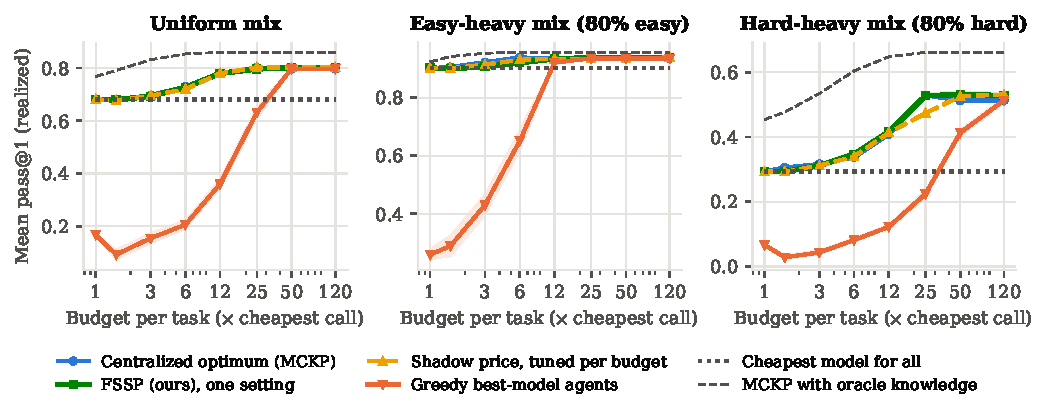
\includegraphics[width=0.9\linewidth]{fig_budget_sweep.pdf}
\caption{Mean realized pass@1 against the budget per task (expected-quality setting, 50 test seeds; shaded bands are 95\% CIs). FSSP with one parameter setting (green) lies on top of the centralized optimum (blue) at every budget and in every mix. Greedy agents (orange) fall below the cheapest-model baseline until the budget covers the frontier model for almost everyone.}
\label{fig:sweep}
\end{figure}

\begin{table}[t]
\centering
\caption{Main comparison (expected-quality setting, full model pool, mean over 3 mixes $\times$ 8 budgets $\times$ 50 test seeds). "Tight" is the mean over budgets $\beta\in\{1.5,3,6\}$. $^*$ = parameter re-tuned for each budget level; FSSP uses one setting.}
\label{tab:main}
\small
\resizebox{\linewidth}{!}{\begin{tabular}{llcccccc}
\toprule
 & Method & Mean pass@1 & Gap (\%) & Gap, tight (\%) & Starved tasks (\%) & Jain & Budget used (\%) \\
\midrule
Centralized & Optimal MCKP (exact ILP) & 0.691 & 0.0 & 0.0 & 0.0 & 0.943 & 84 \\
 & Predictive router & 0.691 & -0.1 & -0.3 & 0.0 & 0.944 & 83 \\
 & Static equal quota & 0.688 & 0.5 & 1.0 & 0.0 & 0.941 & 68 \\
 & Cheapest model & 0.626 & 11.1 & 4.2 & 0.0 & 0.919 & 29 \\
\midrule
Decentralized & \textbf{FSSP (ours)}, random arrival & 0.691 & -0.1 & 0.8 & 0.0 & 0.945 & 67 \\
 & \textbf{FSSP (ours)}, easiest-first & 0.692 & -0.2 & 0.2 & 0.0 & 0.944 & 73 \\
 & FSSP with $\alpha=0$ (fixed price) & 0.678 & 2.6 & 4.9 & 1.5 & 0.940 & 48 \\
 & Shadow price, tuned per budget$^*$ & 0.689 & 0.4 & 0.9 & 0.0 & 0.944 & 69 \\
 & Quasi-linear, tuned per budget$^*$ & 0.680 & 2.7 & 6.0 & 3.4 & 0.938 & 57 \\
 & Shapley share, tuned per budget$^*$ & 0.682 & 2.0 & 4.0 & 1.5 & 0.939 & 54 \\
 & Marginal ratio & 0.515 & 28.1 & 31.4 & 19.9 & 0.872 & 57 \\
 & Greedy best-model & 0.419 & 45.3 & 71.1 & 45.5 & 0.767 & 84 \\
\bottomrule
\end{tabular}}
\end{table}

Figure~\ref{fig:sweep} and Table~\ref{tab:main} show the main result. Greedy agents lose \nnaiveGap\% of the achievable quality on average and \nnaiveGapTight\% at tight budgets, and \nnaiveStarve\% of their tasks receive no model at all. This is the price of anarchy of naive decentralization. FSSP agents, with random arrival and no coordinator, reach a mean pass@1 of \nfsspQ{} against \nmckpQ{} for the exact optimum. Their mean gap is \nfsspGap\% (95\% CI [\nfsspGapLo, \nfsspGapHi]); a small negative gap is possible because MCKP is optimal only for the estimated $\hat q$. No task is starved. Compared with greedy agents, FSSP raises pass@1 by \nfsspVsNaive{} points ($p<\nfsspVsNaiveP$). It is also slightly better than the shadow price that was re-tuned for every budget ($+\nfsspVsDsp$ points, $p=\nfsspVsDspP$), even though FSSP was tuned only once. Its worst single (mix, budget) cell has a gap of \nfsspWorstCell\% (\nfsspWorstCellWhere), compared with \ndspWorstCell\% for the re-tuned shadow price. The centralized router and equal-quota baselines are also close to the optimum, so FSSP pays no measurable price for giving up the central controller.

\subsection{What matters in the decentralized design space}
\label{sec:design}

\begin{figure}[t]
\centering
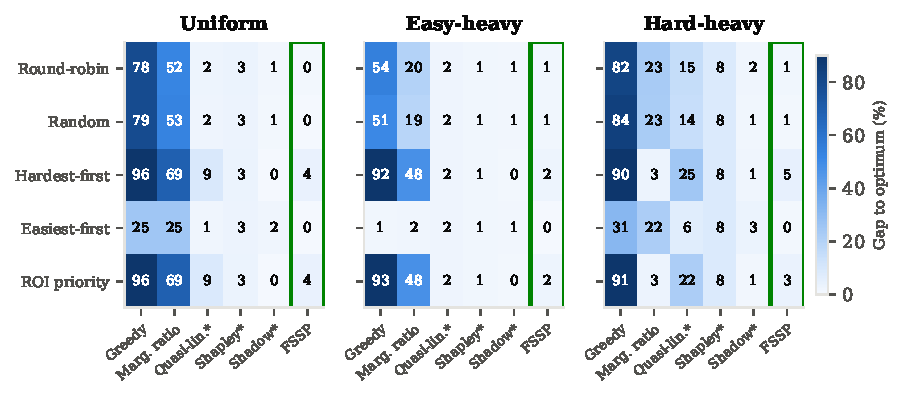
\includegraphics[width=0.9\linewidth]{fig_design_space.pdf}
\caption{Gap to the optimum (\%) for every arrival order $\times$ utility pair, mean over tight budgets. The utility (columns) matters much more than the order (rows). FSSP (framed) is the only column that is close to zero for every order and every mix without per-budget tuning. $^*$ = re-tuned for each budget.}
\label{fig:design}
\end{figure}

Figure~\ref{fig:design} shows the whole design space at tight budgets.

\textbf{Utility first.} Under random arrival, the greedy best-model utility has a gap of \nutbestmodel\% and the marginal-ratio utility \nutmarginalroiratio\%. The ratio utility rewards any affordable upgrade, ignoring what others still need. Price-based utilities reduce the gap to \nutquasilinear\% (quasi-linear$^*$), \nutshapleybudgetshare\% (Shapley$^*$) and \nutdynamicshadowprice\% (shadow price$^*$), but only after re-tuning for each budget.

\textbf{Order second, and the intuitive order is wrong.} Averaged over the utilities, easiest-first has a gap of \narreasiesttaskfirst\% at tight budgets, random \narrrandomfcfs\%, hardest-first \narrhardesttaskfirst\% and marginal-ROI priority \narrmarginalroipriority\%. Hardest-first hands the budget first to the tasks where a dollar buys the least (frontier models solve only about 43\% of hard tasks), and easy tasks that any model would solve starve later. A starved task loses a whole point, an upgrade gains only a fraction. Marginal-ROI priority makes the same mistake, since easy tasks have zero upgrade ROI and are served last. With FSSP the order hardly matters: averaged over all budgets the gap ranges from \nfsspArrMin\% to \nfsspArrMax\% across the five orders. The orders that need no coordinator, random (\nfsspArrrandomfcfs\%) and round-robin FCFS (\nfsspArrfcfs\%), are already at the optimum. Easiest-first (\nfsspArreasiesttaskfirst\%) would need a scheduler that sees the whole queue, a form of central control, and adds almost nothing, so all FSSP results use random arrival.

\subsection{One setting for every budget}

\begin{figure}[t]
\centering
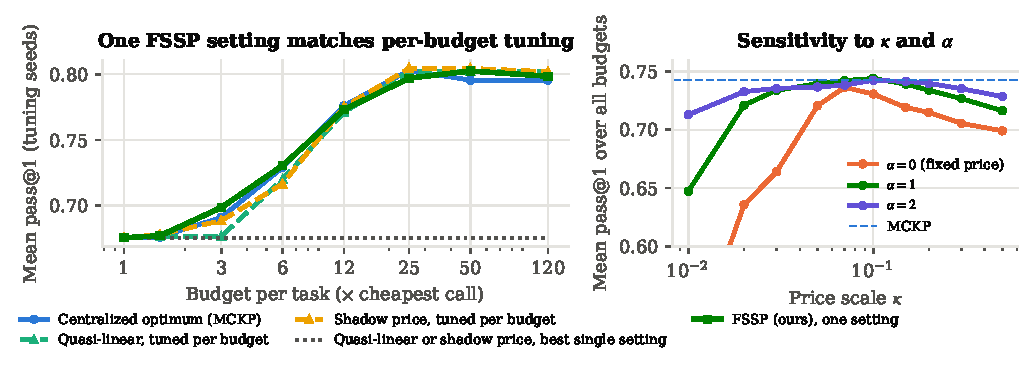
\includegraphics[width=0.8\linewidth]{fig_calibration.pdf}
\caption{Left: on the tuning seeds, quasi-linear and shadow-price utilities match the optimum only when re-tuned for each budget (dashed). Their best single setting (dotted) collapses to the cheapest-model level. FSSP with one setting (green) follows the optimum everywhere. Right: FSSP quality averaged over all budgets is flat over a wide range of $\kappa$ for $\alpha\ge 1$. The fixed-price variant ($\alpha=0$) is more sensitive.}
\label{fig:calib}
\end{figure}

Figure~\ref{fig:calib} explains why FSSP needs no re-tuning. For the quasi-linear and shadow-price utilities, the best price at a budget of $1.5\times$ is wrong by an order of magnitude at $25\times$. Any single value starves tasks at tight budgets or wastes quality at loose ones, so the best compromise is the cheapest model. FSSP's parameter is dimension-free: $\kappa=0.1$ means "an upgrade must raise pass@1 by at least 0.1 per fair share of extra cost", and the optimum is wide and flat for $\alpha\ge1$ (right panel). The scarcity feedback also matters: the fixed-price variant ($\alpha=0$) has a gap of \nalphaZeroGap\% (Table~\ref{tab:main}).

\subsection{Robustness}

\begin{table}[t]
\centering
\caption{Robustness of FSSP with its single parameter setting (random arrival unless stated). Agent-count rows keep 10 tasks per agent and a budget proportional to the number of tasks; noisy-label rows replace a task's tier by a wrong one with probability $\epsilon$; the last rows replace the true $n$ by the online estimate of Section~\ref{sec:unknown-n} or by a fixed wrong forecast. ETF = easiest-first; $^*$ = re-tuned per budget.}
\label{tab:robust}
\small
\resizebox{0.92\linewidth}{!}{\begin{tabular}{lcccccc}
\toprule
 & \multicolumn{2}{c}{Mean pass@1} & \multicolumn{4}{c}{Gap to MCKP (\%)} \\
\cmidrule(lr){2-3}\cmidrule(lr){4-7}
Setting & MCKP & FSSP & FSSP & FSSP+ETF & Shadow price$^*$ & Greedy \\
\midrule
Uniform mix (main setting) & 0.746 & 0.745 & 0.0 & -0.2 & 0.0 & 48.3 \\
Easy-heavy mix (main setting) & 0.926 & 0.923 & 0.4 & 0.0 & 0.3 & 28.1 \\
Hard-heavy mix (main setting) & 0.402 & 0.406 & -0.8 & -0.5 & 0.8 & 59.5 \\
\midrule
Steep pool \{v3.1, r1, gemini-pro\} & 0.691 & 0.693 & -0.5 & -0.5 & 0.1 & 44.3 \\
Oracle information (true pass/fail known) & 0.791 & 0.778 & 2.2 & 1.4 & 7.5 & 16.6 \\
\midrule
$N=5$ agents (budgets $\times$3, $\times$12) & 0.670 & 0.664 & 0.6 & 0.1 & 0.3 & 52.5 \\
$N=20$ agents (budgets $\times$3, $\times$12) & 0.676 & 0.674 & 0.1 & -0.3 & 0.1 & 62.1 \\
$N=50$ agents (budgets $\times$3, $\times$12) & 0.676 & 0.673 & 0.3 & -0.1 & 0.2 & 64.7 \\
\midrule
Correct labels, budgets $\times$3, 12, 50 & 0.758 & 0.759 & 0.0 & 0.0 & -0.1 & 43.9 \\
Noisy difficulty labels, $\epsilon=0.2$ & 0.748 & 0.749 & -0.2 & 0.0 & -0.2 & 43.0 \\
Noisy difficulty labels, $\epsilon=0.4$ & 0.738 & 0.740 & -0.1 & -0.1 & -0.2 & 43.1 \\
\midrule
$n$ unknown: online estimate of $R_k$, no prior & 0.691 & 0.690 & 0.1 & -- & -- & 45.3 \\
$n$ unknown: fixed forecast $2n$ (too high) & 0.691 & 0.671 & 3.7 & -- & -- & 45.3 \\
$n$ unknown: fixed forecast $0.5n$ (too low) & 0.691 & 0.597 & 15.9 & -- & -- & 45.3 \\
\bottomrule
\end{tabular}}
\end{table}

Table~\ref{tab:robust} tests FSSP outside the setting it was tuned on. It stays within about 1\% of the optimum in every mix, in the steeper model pool (gap \nsteepFssp\% where greedy agents lose \nsteepNaive\%), for 5 to 50 agents, and with 20--40\% wrong difficulty labels. Adding agents does not hurt FSSP, because its price depends only on the budget per waiting request. Wrong labels lower the quality of \emph{all} methods: with $\epsilon=0.4$, MCKP loses \nnoiseDropMckp{} points and FSSP \nnoiseDropFssp{} points, so the gap between them does not grow.

The largest gap appears with oracle information (mean \noracleGap\%, worst cell \noracleWorst\% at \noracleWorstWhere). When the true outcome of every task is known, the central planner can match each hard task to the one model that solves it, across the whole batch. A sequential agent cannot see which tasks will come later. Even here FSSP is far better than the re-tuned shadow price (Table~\ref{tab:robust}), whose always-rising price over-taxes late agents.

\textbf{When the number of requests is unknown.} To test the online estimate of Section~\ref{sec:unknown-n}, each request receives a random arrival time in the budget period, and agents see only the clock, the request counter and the remaining budget. With no knowledge of $n$ ($w=0$), online FSSP has a gap of \nunOnlineGap\%, practically the same as FSSP with the true $n$ (\nunKnownGap\%). Starting from a wrong forecast $n_0 = 0.5n$ or $2n$ (weight $w=0.1$) changes little: the gap stays at or below \nunOnlineMaxGap\%, because the observed arrivals soon outweigh the forecast. A \emph{fixed} wrong forecast that is never updated is more harmful, and the two directions fail differently (Table~\ref{tab:robust}). Overestimating the demand ($2n$) makes agents too frugal and leaves money unspent (gap \nunDoubleGap\%, no starvation). Underestimating it ($0.5n$) is worse: once the forecast is used up, each agent believes it is the last one, the price drops to zero, and later requests starve (gap \nunHalfGap\%, \nunHalfStarve\% of tasks starved). In practice the remaining demand should therefore be re-estimated as requests arrive, and when in doubt it is safer to overestimate it.

\subsection{Fairness and first-mover advantage}

\begin{figure}[t]
\centering
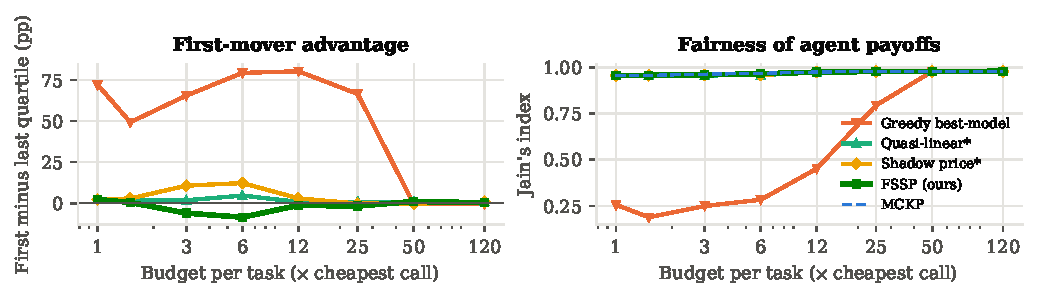
\includegraphics[width=0.8\linewidth]{fig_fairness.pdf}
\caption{Agents arrive in random order and submit all 10 of their tasks at once (uniform mix). Left: payoff of the first quarter of agents minus that of the last quarter, in percentage points (pp) of pass@1. Right: Jain's fairness index over agent payoffs. Greedy agents give the early arrivals almost everything; FSSP is as fair as the central planner.}
\label{fig:fair}
\end{figure}

When agents arrive in random order with all their tasks (Figure~\ref{fig:fair}), greedy agents create a strong first-mover advantage. At tight budgets the first quarter of agents scores \nfmnaive{} points more than the last quarter, and Jain's index falls to \njainnaive. With FSSP the difference is \nfmfssp{} points, i.e. late agents do slightly \emph{better} than early ones, and the Jain index is \njainfssp{}, the same as MCKP (\njainmckp). This is the self-correcting price at work: when early agents leave money unspent, the fair share of later agents grows and their price falls.The re-tuned shadow price keeps a first-mover advantage (\nfmdsp{} points), because its price is lowest for whoever arrives while the pool is still full.

\textbf{When does central control still help?} Centralization keeps an edge only through extra \emph{information}. Knowing the true outcome of every task raises the optimum by \ninfoGainMin--\ninfoGainMax{} points of pass@1, far more than the coordination gap of FSSP. The confidence cascade, which runs unit tests after each call and escalates on failure, reaches \ncascadeQ{}, \ncascadeGap\% above MCKP with estimated qualities. Both kinds of information could also be given to decentralized agents, for example an FSSP agent that retries after a failed test.

% ======================================================================
\section{Limitations and Conclusion}
\textbf{Limitations.} (i) The difficulty tiers are computed from the models' own results ("easy" means all six models passed), which gives agents a cleaner signal than a real classifier would. The noisy-label test shows the comparison is robust, but absolute qualities are optimistic. (ii) Costs are mean costs per model, not per-task token costs. (iii) The online demand estimate assumes requests arrive at a roughly constant rate over the budget period; bursty or seasonal traffic would need a better forecast. (iv) We use one benchmark (code generation); other domains and price ladders should be tested.

\textbf{Conclusion.} Many LLM agents can share one budget without a central controller. Greedy decentralized selection wastes most of the budget and starves late agents, and price-based utilities fix this only if someone re-tunes the price for every budget. Fair-Share Shadow Pricing solves both problems with one line: each agent prices money by the inverse of the budget still available per request still to come. With one parameter setting, FSSP agents match the exact centralized knapsack optimum on held-out data, never starve a task in the realistic setting, and are as fair as the central planner. They need no scheduler, and they do not need to know the number of requests in advance. Central control remains useful only when it brings information the agents lack, such as known task outcomes or test feedback.

% ======================================================================
\section{Contribution}

\begin{table}[H]
\centering
\footnotesize
\caption{Division of work and completion status.}
\label{tab:contrib}
\begin{tabular}{l p{11.4cm} c}
\toprule
\textbf{Member} & \textbf{Assigned tasks} & \textbf{Status} \\
\midrule
Chauhan Mitesh & Dataset preparation (LLMRouterBench conversion, difficulty mixes, audit); centralized approaches (MCKP, router, cascade, quota, cheapest). & Fulfilled \\
Rathod Yuvraj  & Problem formulation, experiment setup, code structure; experimental evaluation, design and testing of FSSP; writing this report. & Fulfilled \\
Solanki Viraj  & Utility functions for the decentralized approaches (quasi-linear, shadow price, Shapley share, marginal ratio). & Fulfilled \\
Sunay Desai    & Arrival-ordering policies and their integration with the utilities in the sequential game. & Fulfilled \\
\bottomrule
\end{tabular}
\end{table}

\textbf{Code and reproduction.} The repository \texttt{README.md} gives the setup, exact commands and screenshots of all result plots and tables. Every table and number in Section~\ref{sec:results} is written to \texttt{report/generated/} by \texttt{scripts/hypotheses/paper\_figures.py} from the raw runs in \texttt{results/hypotheses/}.

{\footnotesize
\bibliographystyle{unsrt}
\bibliography{references}
}

\end{document}
